%%%% LAST UPDATED: 12/3/2017 - CRG
\documentclass[12pt,addpoints]{exam} 
\usepackage{amssymb, amsthm, amsmath, amscd, amsfonts}
\usepackage{graphicx}
\usepackage{verbatim}
\usepackage[all]{xy}
\usepackage{pgf,tikz}
\usetikzlibrary{arrows}
\usepackage[margin=.5in,bottom=1in]{geometry}
\usepackage{enumitem}
\usepackage{hyperref}
\usepackage{ifthen}
\usepackage{wrapfig}
\usepackage{subcaption}
\usepackage[stamp=false]{draftwatermark}
\SetWatermarkText{\copyright2026 Courtney Gibbons All Rights Reserved}
\SetWatermarkScale{1.5}

%% PARAMETERS FOR SETTING DATES, CLASS, ETC
\newcommand{\semester}{Spring 2026}
\newcommand{\coursename}{Decisions by Design}
\newcommand{\coursenumber}{{\tt Math 260}}
\newcommand{\examname}{Midterm 1}
\newcommand{\examdate}{March 10, 2026}
\newcommand{\honorcourtstudent}{the Chair of the Honor Court}
\newcommand{\deanofstudents}{the Associate Dean of Students}

%% Augmented Matrix Environment
\newenvironment{amatrix}[1]{%
	\left[\begin{array}{@{}*{#1}{r}|r@{}}
	}{%
	\end{array}\right]
}

\newcommand{\ZZ}{\mathbb Z}       
\newcommand{\NN}{\mathbb N}   
\newcommand{\QQ}{\mathbb Q}
\newcommand{\RR}{\mathbb R}    
\newcommand{\ds}{\displaystyle}
\newcommand{\defi}[1]{\textbf{\textit{#1}}}

\DeclareMathOperator{\RREF}{RREF}

\setlength\linefillheight{.3in}

\begin{document}
\thispagestyle{empty}
%%%%%%%%%%%%%%%% NAME + HONOR CODE BLOCK %%%%%%%%%%%%%%%%%%
\noindent Name: \hrulefill\\[1em]
%& & \\
%%& & Instructor: \underline{\hspace{2.3in}}\\[1em]


\bigskip

\noindent\hrulefill
\bigskip
%%%%%%%%%%%%%%%%% HEADER BLOCK %%%%%%%%%%%%%%%%
\begin{center}
\large \textsc{\coursename} \\
\smallskip
\normalsize \coursenumber\ --- \examname\ --- Wildfires\\
\smallskip
\examdate
\end{center}
\bigskip
\hrule


\vspace{20pt}

\noindent This exam is double-sided with \numpages\ pages and a total of \pointsinrange{all} points. You should complete this exam in 75 minutes (assuming no accommodations). There is extra room for scratch work on pages 6 and 7 of the exam.\\


\noindent \textbf{About this Exam.}
\begin{itemize}
  \setlength{\itemindent}{-1em}
  \item The only technologies you may use are a pen or pencil, the printed pages of this exam, scratch paper, and a calculator (you can use your phone as long as it is in airplane mode and you access nothing other than the calculator).
	\item Read each question and its instructions carefully.
	\item Use scratch paper as needed before writing on the exam.
	\item On the exam pages, show your work neatly and in an organized fashion. Only work on these pages will be graded.
	\item If there is a box or line for a final answer, please put your final answer in the box or on the line.
	\item If there is a bubble choice for your answer, please fill in the bubble. Sometimes there is more than one answer to this kind of question; fill in every choice that is correct.
  \item Sign the honor code below when you finish the exam.
\end{itemize} 

\vspace{15pt}

\hrule

\vspace{12pt}

\noindent I have neither given nor received unauthorized help. I have not used unauthorized resources. I have adhered to the time limit (within 5 minutes).\\[3em] Signed, \hrulefill\\[1em]

\vfill

Turn in your Midterm and Exam Packet; make sure your name is on both!

\clearpage

\begingradingrange{all}

\section*{Part I. Mathematical Modeling}

	The exam packet provides a Mathematical Modeling Brief describing an intervention to solve a problem (Step 6 - Reporting the Results). For each of the other five steps in the M3 Mathematical Modeling Process, describe how the step is playing out or indicate that you don't have enough information from the report to do so. Underline the parts of the text you are using to inform your answers.
	  	
	\begin{questions}
		\question[5] 
			(Defining the Problem Statement) What problem are researchers trying to solve?
			\vfill

  	\question[5] 
  		(Making Assumptions) What assumptions are they making to reduce complexity?
  		\vfill

		\question[5] 
			(Defining Variables) What variables have the researchers identified as being of primary importance to the problem?
			\vfill

		\question[5] 
			(Getting a Solution) What type of model and/or tools are the researchers using to solve the problem?
			\vfill

		\question[5] 
			(Analysis and Model Assessment) What are the researchers doing to understand how well the model works to solve the problem?
			\vfill
	\end{questions}

\clearpage

\section*{Part II. Apportionment}

	% \begin{wrapfigure}{l}{.4\textwidth}
	% 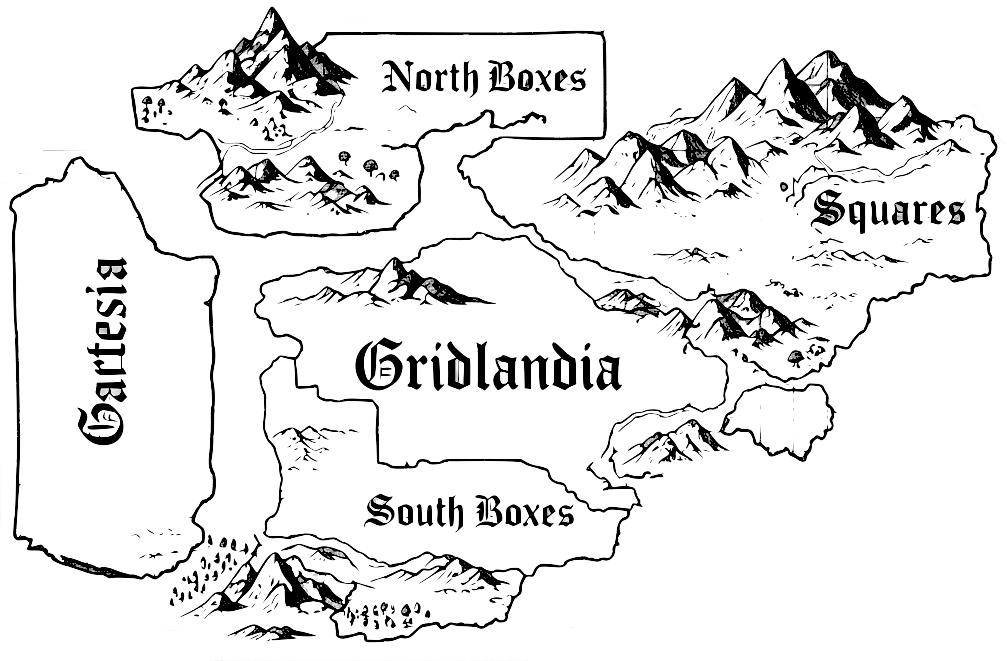
\includegraphics[width=\linewidth]{graphpapyra.jpeg}
	% \end{wrapfigure}

	Welcome to Flatland! In Flatland, the Unified Republic of Graphpapyra (URG, or ``urg'' as they call themselves; pop.\ 27000) is a country that has a representative system of government. URG has four states: Cartesia (pop.\ 10290), Gridlandia (pop.\ 1900), the Commonwealth of Squares (pop.\ 6100), and North Boxes (pop.\ 8710).\footnote{South Boxes (pop.\ 2845) seceded following an uncivil war.}\\
	
	Although life is fairly simple in Flatland and URG, residents still face problems we recognize from our lives, like the problem of allocating representatives for these four states based on their populations. Their legislative body, the URG Assembly (URGA or ``urg-guh'') has 100 seats.


	\begin{questions} \setcounter{question}{5}
		\question[3] 
			Based on the information above, the standard divisor is	\fillin[270].

		\question[5] 
			Complete Table~\ref{tab:four_states} in the Exam Packet to apportion the seats by Hamilton's method (every gets their lower quota; biggest decimal remainders are awarded the extra seats).

		\question[2] 
				Webster's method uses traditional rounding ($n \geq 0.5$ rounds to $n+1$, $n < 0.5$ rounds to $n$) with a divisor that ensures the rounded numbers sum to 100. Does the standard divisor lead to a valid Webster's apportionment?
				%
				\begin{oneparcheckboxes}
					\choice Yes
					\choice No
				\end{oneparcheckboxes}

		\question[5] 
			South Boxes sees that life in URG has been steadily improving and decides to return to the Republic with its 2845 residents. The URGA adds 10 news seats to accommodate their return. Compute the new apportionment in Table~\ref{tab:five_states}.

		\question[5] 
			One of the Squares assembly members is unhappy and tries to convince URGA to use Webster's method with a modified divisor of 271. Compute the propossed apportionment in Table~\ref{tab:five_states_with_modified_divisor}, then explain why this would threaten the fragile reunification.
			\vfill

			\begin{flushleft}
				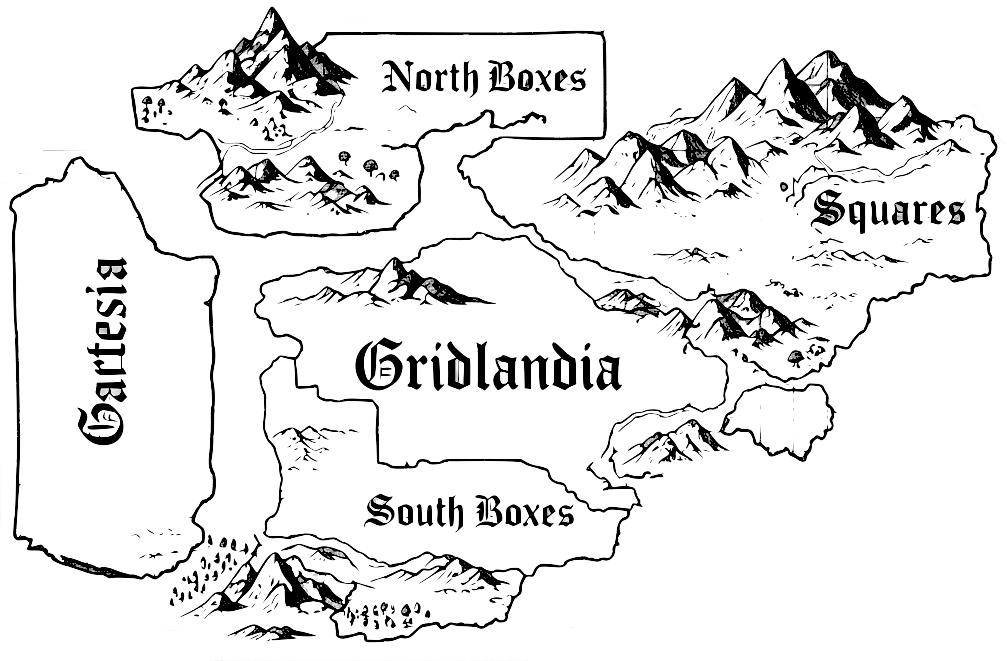
\includegraphics[width=.6\linewidth]{graphpapyra.png}
			\end{flushleft}

	\end{questions}

\clearpage

{
	\newgeometry{margin=1.5cm} \thispagestyle{empty}

	}

\restoregeometry
\clearpage

\section*{Part III. Districting Questions}

	In the Exam Packet, you will find grids relating to this question.\\

	It's time for redistricting in URG! By precinct, voters prefer the Clubs Party or the Hearts Party.\footnote{Conveniently, the populated region of Gridlandia is a 7$\times$7 grid.}\\

	In the MidSouth, there is a minority voting bloc indicated with large hearts. URG and Gridlandia laws dictate that these voters must have an opportunity district where their views are in the majority.\\

	To ensure fairness, Gridlandia has created a task force to analyze proposed district maps. The task force runs an MCMC analysis of district plans given the distribution of voter preferences in prior elections which returns the following distribution:

	\fullwidth{
		\begin{center}
			\begin{tikzpicture}[y=0.05cm]
				%
				% macro: bar at position, height, label
				\newcommand{\barval}[4]{
				  \draw[fill=gray!30] (#1,0) rectangle (#1+0.8,#2);
				  \node at (#1+.4,#2+4) {#3};
				  \node at (#1+.4,-4) {#4};
				}
				%
				\barval{0}{22}{217}{\scriptsize{0 seats}}
				\barval{1.2}{57}{566}{\scriptsize{1 seats}}
				\barval{2.4}{21}{205}{\scriptsize{2 seats}}
				\barval{3.6}{1.2}{12}{\scriptsize{3 seats}}
				\barval{4.8}{.1}{0}{\scriptsize{4 seats}}
				\barval{6}{.1}{0}{\scriptsize{5 seats}}
				\barval{7.2}{.1}{0}{\scriptsize{6 seats}}
				\barval{8.4}{.1}{0}{\scriptsize{7 seats}}
				%
				\draw[thick] (-.5,0) -- (9.8,0);
				\node at (5,-12) {$\heartsuit$ seats};
			\end{tikzpicture}
		\end{center}
	}

	\begin{questions}\setcounter{question}{10}
					
		\begin{minipage}{.5\textwidth}
					\question[5] 
						Compute the number of seats each party wins in the district plans on the last page. \emph{You will complete Plan 1$^\prime$ in a later question; compute the numbers of seats when your plan is complete.}
		\end{minipage}\hfill
			% 
		\begin{minipage}{.4\textwidth}
				{
					\renewcommand{\arraystretch}{1.5}
					\begin{tabular}{|c|c|c|c|c|c|}
						\hline
						Plan & 1 & 2 & 3 & 4 & 1$^\prime$ \\
						\hline
						$\clubsuit$ seats & \phantom{100} & \phantom{100} &  \phantom{100} & \phantom{100}& \phantom{100} \\
						\hline
						$\heartsuit$ seats & & & & & \\
						\hline
					\end{tabular}
				}
		\end{minipage}

		\question[1] 
			Based on the distribution above, the task force will reject one of the plans on the next page. Which one?
			%
			\begin{oneparcheckboxes}
				\choice Plan 1 \choice Plan 2 \choice Plan 3 \choice Plan 4
			\end{oneparcheckboxes}

		\question[1] 
			Based on the law protecting the right of representation for minority voting blocs, which plans will the task force reject?
			%
			\begin{oneparcheckboxes}
				\choice Plan 1 \choice Plan 2 \choice Plan 3 \choice Plan 4
			\end{oneparcheckboxes}

		\question[3] Plan 1 can be modified to create an opportunity district by modifying districts 5 and 7. Do so on the grid labeled Plan 1$^\prime$ on the next page.

\clearpage

		\fullwidth{Define $p(D)$ to be the perimeter of a district $D$, $a(D)$ to be the area of a district $D$, and $MP(D)$ is the minimal convex polygon containing $D$.}
	
		\question[5] 
			Compute \textit{and interpret} the Polsby-Popper score for $D_{3,3}$ (Plan 3 District 3),\\[.5em]
			\(\displaystyle \mathrm{polpop}(D_{3,3}) = \frac{4\pi a(D_{3,3})}{p(D_{3,3})^2}.\)
			\vfill

		\question[5] 
			Compute \textit{and interpret} the convex polygon score for $D_{1,6}$ (Plan 1 District 6),\\[.5em] \(\displaystyle \mathrm{convex}(D_{1,6}) = \frac{a(D_{1,6})}{a(MP(D_{1,6}))}.\) 
			\vfill

		\question[5] 
			Compute the Efficiency Gap for Plan 2 by completing the table below, where\\ \(\mathrm{EG} = \dfrac{ \mathrm{wasted}(\clubsuit) - \mathrm{wasted}(\heartsuit)}{49}.\)\hfill EG = \fillin[eg]

			A wasted vote in a district is a vote for the losing candidate or a vote for the winning candidate that was unneeded.

			\begin{center}
				\renewcommand{\arraystretch}{1.75}
				\begin{tabular}{|c|c|c|c|c|c|}
					\hline
					District & $\clubsuit$ votes &	$\heartsuit$ votes &	Winner &	$\clubsuit$ wasted votes	& $\heartsuit$ wasted votes \\
					\hline
					1 & 4 & 3 & $\clubsuit$ & 0 & 3 \\
					\hline
					2 & & & & & \\
					\hline
					3 & & & & & \\
					\hline
					4 & & & & & \\
					\hline
					5 & & & & & \\
					\hline
					6 & & & & & \\
					\hline
					7 & & & & & \\
					\hline 
					totals: & & & & & \\
					\hline
				\end{tabular}
			\end{center}
	\end{questions}

\endgradingrange{all}
\clearpage

this page intentionally left (mostly) blank

\clearpage

		\input{MIDTERM1-packetC}
\end{document}